Figures~\ref{fig:rewrite-rsi-accumulation}--\ref{fig:rewrite-rsi-distribution}
use the same four elasticities and show two time windows. The first includes
two pre-event years, followed by the first ten years after activation;
the second covers years 10--500. The pre-event segments are the analytical
fixed-productivity BGPs. The post-event segments are separately solved
equilibrium approximations subject to the admission checks in
Appendix~\ref{app:rewrite-algorithm}. The vertical line at zero marks RSI
activation. Vertical scales differ across windows so that early adjustment
does not hide the subsequent dynamics.

The continuity of output does not imply continuity of its growth rate.
Immediately after activation, output-per-person growth is approximately
$4.60\%$, $11.51\%$, $13.48\%$, and $23.97\%$ across the four elasticities,
compared with $1\%$ before activation. These are instantaneous annual rates,
not realized growth over a calendar year. The price target produces a rapid
initial response even though the economy begins on its pre-RSI BGP.
Removing the change in production weights therefore removes the level jump,
not the sensitivity of growth to the assumed pace of RSI.

\begin{figure}[H]
 \centering
 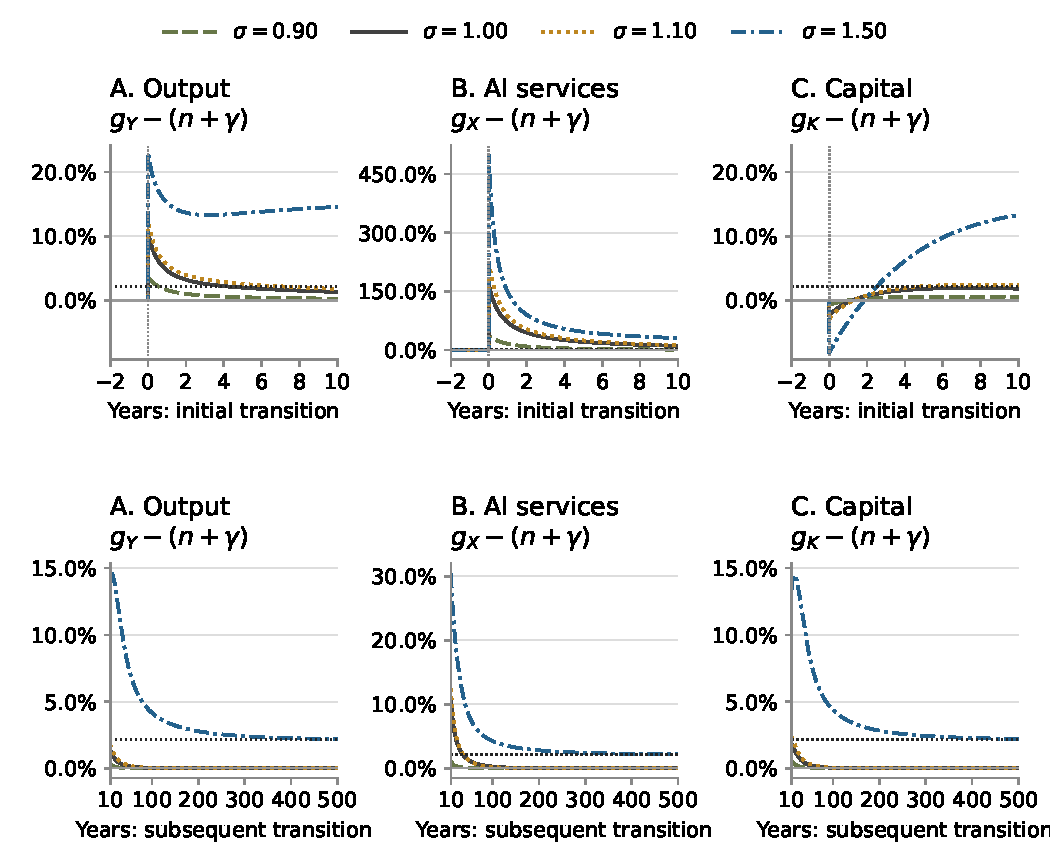
\includegraphics[width=\textwidth]{figures_rewrite/equilibrium_rsi_activation_accumulation_growth_windows.pdf}
 \caption{RSI activation: growth of output, AI production services, and
 capital per unit of effective labor. Rates are instantaneous annual rates.
 The upper row includes the pre-event BGP and years 0--10; the lower row
 shows years 10--500. Panels A and C share a scale within each row.
 Dotted horizontal lines show the analytical limits for $\sigma=1.50$.}
 \label{fig:rewrite-rsi-accumulation}
\end{figure}

All four interest rates start at $5\%$. The three labor-supported economies
eventually return to $5\%$, with output per person and real wages growing
at $1\%$. At $\sigma=1.50$, the limiting interest rate is approximately
$7.13\%$, output-per-person growth is $3.13\%$, and real-wage growth is
$2.42\%$. The higher wage-growth rate is accompanied by an even higher
output-growth rate and a vanishing labor income share. The transition can
overshoot these limiting growth and interest rates.

\begin{figure}[H]
 \centering
 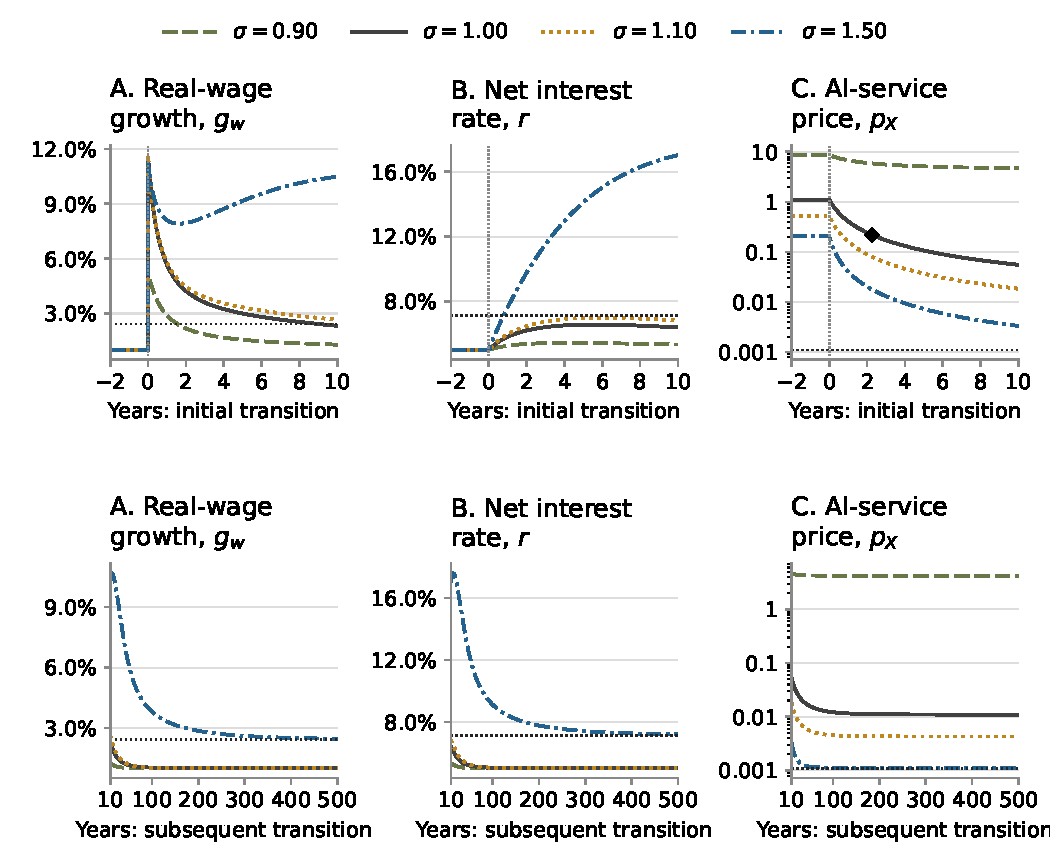
\includegraphics[width=\textwidth]{figures_rewrite/equilibrium_rsi_activation_growth_returns_windows.pdf}
 \caption{RSI activation: real-wage growth, the net interest rate, and
 the AI-service price. Wage growth and interest rates are annual; the
 price is in final-good units on a logarithmic scale. The diamond marks
 the unit-elastic price target at 2.25 years. The vertical line marks
 activation; dotted horizontal lines show the $\sigma=1.50$ limits.}
 \label{fig:rewrite-rsi-prices}
\end{figure}

The prospect of higher future income affects spending at activation. Consumption
jumps by approximately $2.85\%$, $9.29\%$, $10.80\%$, and $22.71\%$,
respectively, while research starts from zero. Since current output and
inference use do not jump, each additional unit of consumption or research
reduces current investment in physical capital by one unit. Capital per
unit of effective labor initially falls in all four cases.

The high-substitution case makes the resource requirement particularly
clear. Research initially absorbs $9.32\%$ of output, or $181.1\%$ of
AI-industry revenue, and the developer's net profit is $-6.02\%$ of output.
Gross investment, $Y-C-U-M$, is initially $-6.09\%$ of output. This
requires disinvestment of the model's reversible one-good capital, not
merely transfers to the developer. Requiring nonnegative gross investment
would change the equilibrium problem. Financing developer losses and
satisfying the economy's resource constraint are distinct requirements.

\begin{figure}[H]
 \centering
 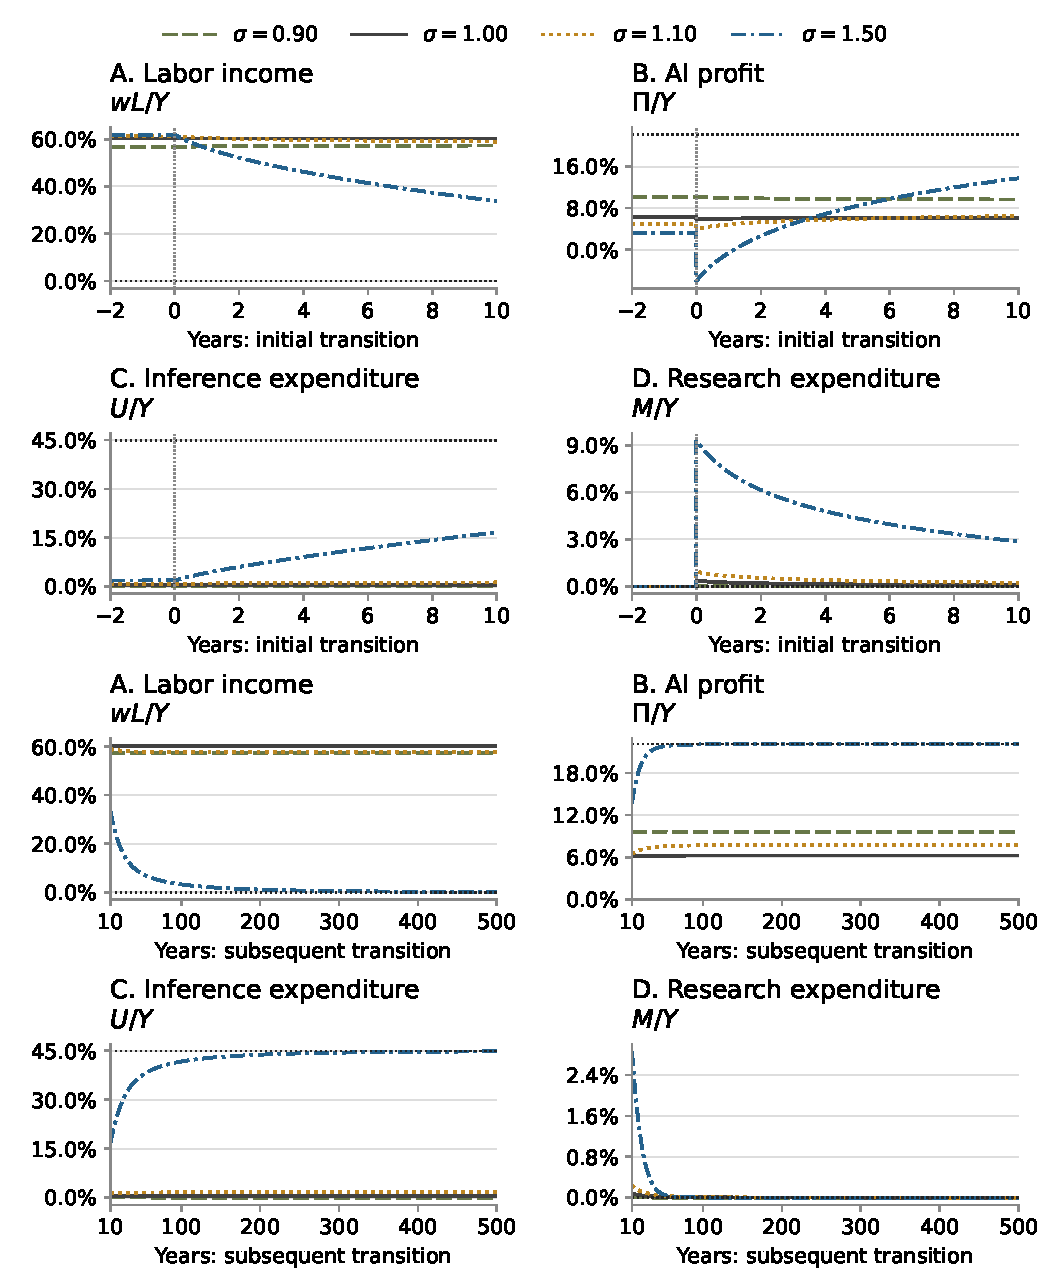
\includegraphics[width=\textwidth]{figures_rewrite/equilibrium_rsi_activation_ai_distribution_windows.pdf}
 \caption{RSI activation: labor income, AI net profit, inference expenditure,
 and research expenditure relative to output. The first two rows show the
 pre-event BGP and years 0--10; the last two show years 10--500. Research
 is zero before activation, while pre-event AI operating profit is positive.
 The omitted gross capital share remains $\alpha=0.33$.}
 \label{fig:rewrite-rsi-distribution}
\end{figure}

Matching the initial capital--output ratio does not match the initial size
of the AI sector. Its revenue initially represents approximately $10.26\%$,
$6.70\%$, $5.79\%$, and $5.15\%$ of output across the four elasticities.
These are model outcomes, not empirical targets. In particular, at unit
elasticity revenue's share equals $(1-\alpha)\omega_X$, so changing $K_0$,
$B_0$, or $\chi$ cannot adjust that share. The exercise isolates the
activation of RSI from an instantaneous change in production technology;
it is not a complete empirical calibration of the current AI industry.
